\documentclass[tikz]{standalone}
\usepackage{fontspec}
\usepackage{tikz}
\usetikzlibrary{arrows.meta, positioning, shapes.geometric}

\setmainfont{Iosevka Nerd Font} 

\begin{document}

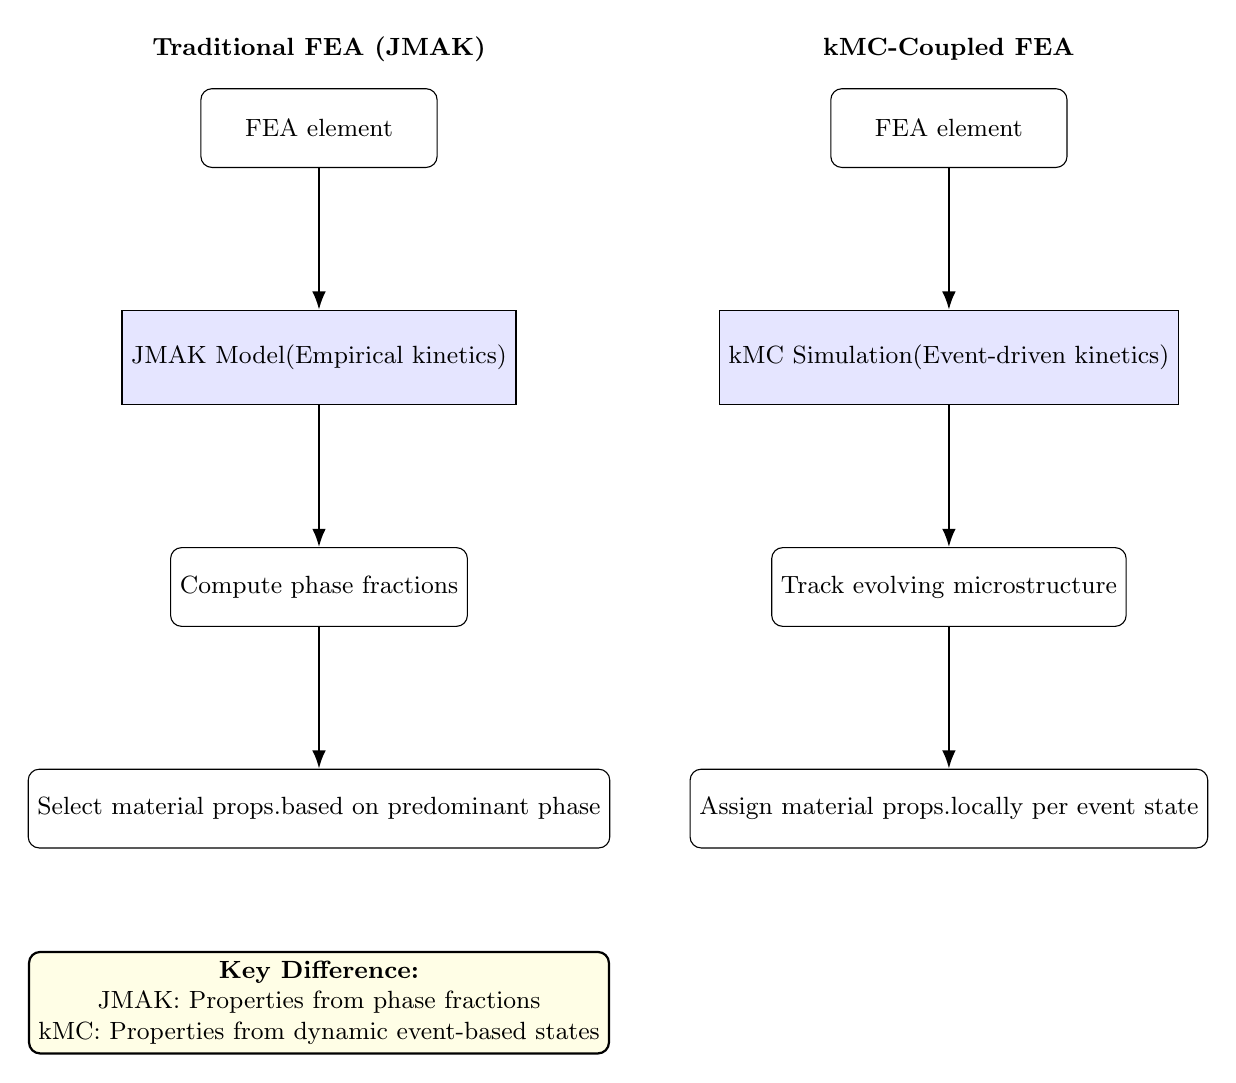
\begin{tikzpicture}[
    node distance=1.8cm and 2.2cm,
    box/.style={rectangle, draw, rounded corners, minimum width=3cm, minimum height=1cm, text centered},
    process/.style={rectangle, draw, minimum width=3.2cm, minimum height=1.2cm, text centered, fill=blue!10},
    phase/.style={rectangle, draw, minimum width=1.5cm, minimum height=0.8cm, fill=gray!20},
    arrow/.style={-{Latex}, thick},
	font=\small
]

% Titles
\node[align=center] at (-4, 4.5) {\textbf{Traditional FEA (JMAK)}};
\node[align=center] at (4, 4.5) {\textbf{kMC-Coupled FEA}};

% JMAK branch
\node[box] (fea1) at (-4, 3.5) {FEA element};
\node[process, below=of fea1] (jmak) {JMAK Model\\(Empirical kinetics)};
\node[box, below=of jmak] (phase1) {Compute phase fractions};
\node[box, below=of phase1] (mat1) {Select material props.\\based on predominant phase};

% Arrows
\draw[arrow] (fea1) -- (jmak);
\draw[arrow] (jmak) -- (phase1);
\draw[arrow] (phase1) -- (mat1);

% kMC branch
\node[box] (fea2) at (4, 3.5) {FEA element};
\node[process, below=of fea2] (kmc) {kMC Simulation\\(Event-driven kinetics)};
\node[box, below=of kmc] (phase2) {Track evolving microstructure};
\node[box, below=of phase2] (mat2) {Assign material props.\\locally per event state};

\draw[arrow] (fea2) -- (kmc);
\draw[arrow] (kmc) -- (phase2);
\draw[arrow] (phase2) -- (mat2);

% Optional legend
\node[draw, thick, rounded corners, align=center, minimum width=7cm, below=1.3cm of mat1, fill=yellow!10] (legend) {
  \textbf{Key Difference:}\\
  JMAK: Properties from phase fractions\\
  kMC: Properties from dynamic event-based states
};

\end{tikzpicture}

\end{document}
